\subsection{Implementierung}

Im folgenden Abschnitt wird auf die Implementierung der Funktionen des Transportroboters eingegangen. Dabei werden die zwei Teilabschnitte, die Implementierung der Navigation und die Implementierung der Paketübergabe, betrachtet. Der Großteil der Implementierung wurde in den ROS-Packages „epos2-control“ und „simple-navigation-goals“ realisiert.

\subsubsection{Ablaufkonzept}

Die Abbildung \ref{fig:Ablaufkonzept} gibt einen Überblick über die implementierten Funktionen und deren Ablaufreihenfolge bei dem Transport von Paketen. Nach dem Eingang eines Auftrages über das MICAz-Modul wird dieses in ein Navigationsziel umgesetzt. Neben der Position auf der Umgebungskarte wird auch die Zielhöhe des Hubs dem Auftrag entnommen. War die Navigation zur Zielposition und die Steuerung des Hubs erfolgreich beginnt die Förderbandsteuerung je nach Auftrag mit dem Be- bzw. Entladen. Die Auswertung der Lichtschranken der Fördereinheit ermöglicht die Zustandserkennung der Paketübergabe. Nach erfolgreicher Übergabe ist der Volksbot bereit ein folgendes Ziel anzufahren oder einen neuen Auftrag entgegenzunehmen.

\begin{figure}[h!]
 \centering
		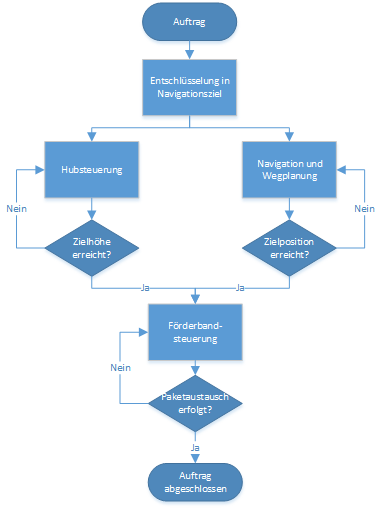
\includegraphics[width=1\textwidth]{drive/Ablaufkonzept.png}
	\caption{Ablaufkonzept}
	\label{fig:Ablaufkonzept}
\end{figure}


\subsubsection{Implementierung der Navigation}
Nach erfolgreicher Inbetriebnahme der Hardware des Volksbots wurde die Odometrieberechnung anhand der zurückgelegten Strecke der Räder implementiert. Die Berechnung der zurückgelegten Wegstrecke und der Drehung des Roboters erfolgt über folgende Formeln\cite[S. 1]{Der:2000}:

\begin{equation}
\triangle s = \dfrac{\triangle R + \triangle L}{2}
\end{equation}
 
\begin{equation}
\triangle \alpha = \dfrac{\triangle R - \triangle L}{D}
\end{equation} 

Die Daten der Wegstrecke und der Drehung des Roboters werden genutzt, um mit folgenden Formeln die x- und y-Position des Roboters zu berechnen:

\begin{equation}
x = x(t-1) + (\triangle s * \cos (\alpha (t-1) + \triangle \alpha))
\end{equation} 

\begin{equation}
y = y(t-1) + (\triangle s * \sin (\alpha (t-1) + \triangle \alpha))
\end{equation} 

Der Drehwinkel des Roboters ergibt sich aus der Addition des vorherigen Winkels mit der zuletzt durchgeführten Änderung des Drehwinkels.

\lstinputlisting[language=C++, style=customc, captionpos=b, caption={Implementation der Odometrieberechnung}, label=lst:odom]{src/drive/lst/Odometrie.cpp}

Die Daten der Odometrie werden zur Lokalisierung des Roboters innerhalb einer mit dem SICK LMS100 Laserscanners erstellten Umgebungskarte verwendet. Die Implementierung erfolgte ebenso wie bei der Entwicklung der Treiber im „epos2-control“-Package. Bei der Erstellung der Umgebungskarte wurde auf das „Gmapping“-Package von ROS zurückgegriffen. Der darin enthaltene Algorithmus nutzt die Daten des Laserscanners, um während der Fahrt des Roboters aus seiner erfassten Umgebung eine Karte zu erstellen. Zur Visualisierung der Karte und der Daten des Laserscans wurde „Rviz“, ein Visualisierungstool innerhalb der ROS-Umgebung verwendet. Mit Hilfe von Rviz ist es neben der Visualisierung unter anderem möglich die initiale Position des Roboters, sowie Navigationsziele innerhalb der Karte festzulegen. (Screenshot Rviz) Mit dem Ziel den auftretenden Abweichungen der Odometrieberechnung entgegenzuwirken, wurde das „adaptive Monte Carlo Localisation“-Package (AMCL) implementiert. Vereinfacht formuliert, nutzt dieses Verfahren die Daten des Laserscans und der Karte, um mit Hilfe der Merkmale des aktuellen Scans und der zugrundeliegenden Daten der Kartenrepräsentation eine Schätzung der Position des Roboters auszuführen. \cite[S. 6]{Bischoff:2004}
Eine funktionsfähige Selbstlokalisation ist die Grundlage für eine erfolgreiche autonome Navigation in der Umgebung des Roboters. Das ROS-Framework stellt mit dem „move-base“-Package die nötigen Funktionen für die Navigation bereit. Das Package hat den Dijkstra-Algorithmus zur Wegplanung implementiert und nutzt zwei parametrisierbare Costmaps, um Eigenschaften wie z.B. den Mindestabstand zu Hindernissen oder das Verhalten bei Planungsfehlern festzulegen. Nach der Planung des Weges werden automatisch die passenden Steuerbefehle generiert. Falls der Volksbot in eine unvorhergesehene Situation gerät und seine geplante Route nicht mehr gültig ist, kommen Rettungs-Funktionen des Packages zum Einsatz. Dabei wird eine Rotation um die eigene Achse des Roboters durchgeführt, um einen geeigneten neuen Weg zu finden. Durch die Anpassung von Ziel-Toleranzen kann das Verhalten des Roboters in der Nähe der Zielposition beeinflusst werden. Je geringer die Toleranzen, desto länger benötigt der Roboter die gewünschte Position einzunehmen.

\subsubsection{Implementierung der Paketübergabe}
Damit der Austausch der Pakete mit den Komponenten des Materialflusses erfolgen kann, musste die Kommunikation über die MICAz-Module und Automatismen zur Anpassung der Hub-Position an die Höhe der jeweiligen Rampe implementiert werden. Nachdem ein Auftrag vom Materialfluss empfangen wurde, wird die Annahme des Auftrags dem Materialfluss bestätigt und der Auftrag in ein passendes Navigationsziel auf der Umgebungskarte umgesetzt. Für den Prozess des Entschlüsselns von den Nachrichten des Materialflusses wurde das ROS-Package namens „Simple-Navigation-Goals“ implementiert. Neben der Umsetzung von Navigationszielen sendet dieses Package ROS-interne Nachrichten, welche Informationen über die gewünschte Position des Hubs und das Erreichen der Zielposition enthalten.
Sobald die Zielposition erreicht wurde, beginnt die Hubsteuerung mit der Anpassung der Hubposition an die geforderte Höhe. Anschließend folgt eine Benachrichtigung an den Materialfluss und das Förderband wird in Gang gebracht. Die Auswertung der Lichtschranken bewirkt den Haltevorgang des Förderbands und das nächste Navigationsziel wird festgelegt.


